\chapter{OPTIMAL INTERPOLATION TO IMPROVE SATELLITE NOWCASTS WITH DATA}
\label{chap:satoi}

references to other sections
- application
- basic background
- results

\section{Satellite to Irradiance Algorithms}
- high res requirements
- GOES, time res

\subsection{UASIBS Model}
The University of Arizona Solar Irradiance Based on Satellite (UASIBS)
model was developed at by Chang Ki Kim in 2015 \citep{Kim2016}.
This model relies on the infrared images of the GOES-W satellite to
find completely overcast areas based on a comparison of the brightness
temperature difference (difference between 10.7 and 3.9 $\mu$m
images) to a reference calculated over the past few weeks.
If the infrared channels do not find an area to be overcast, the
visible image is compared to a threshold image to determine if any of
the 16 pixels in the 4km $\times$ 4km box have a cloud.
Once pixels are classified as cloudy or clear, a look-up table is
employed to find the atmospheric transmittance and GHI on the ground
for each pixel.
A number of look-up tables are generated from using Goddard Space
Flight Center Radiative Transfer Model: one for clear sky
accounting for aerosols, one for high level clouds, one for mid level
clouds, one for low clouds, and one for cumulus clouds.

While the cloud detection routine seems to function well, the look-up
table approach to calculate transmittance is limited.
First, a number of climatological averages, specific to Tucson, are
used in the calculations of the look-up tables including AOD and
ozone.
Instead, near real-time analysis and forecasts of AOD and ozone are
available from Monitoring atmospheric composition and climate (MACC)
project \citep{Morcrette2009} and a ground truth measurement of AOD is
available from the Tucson AERONET site \citep{Holben1998}.
Another limitation is that only ten values of the solar zenith angle
are used which introduces artificial steps noticable in the output
GHI.
With newer, fast radiative transfer codes, perhaps the look-up table
approach can be replaced with a direct call to a radiative transfer
code to avoid this issue.

\subsection{Empirical Model}
- based on suny
- improvments to be made

\subsection{Other Models}
gsip
nsrdb alg

\subsection{Future Models}
goes 16


\section{Parameter Estimation}
\label{sec:paramopt}
Section 6 of \cref{app:satoi} discusses the tuning of OI for a
specific location including the estimation of the parameters
$k,\: l,\: d$ by minimizing the mean-squared error (MSE) of the
analysis over sensors withheld from OI.
To perform this minimization a grid search over the parameters was
performed and the resulting MSE for each set of parameters is shown in
\cref{fig:paramopt}.
This figure clearly shows distinct minima in parameter space for the
UASIBS satllite to irradiance model which indicates that  OI is
sensitive to the choice of parameters.
On the other hand, the lack of distinct minima in parameter space for
the empirical model indicates that a wide range of parameters would
give similar results after performing OI.
If in the future the empirical model is chosen as the background model
for an OI based routine, a more thorough investigation into why OI is
insensitive to these parameters is warranted.

\begin{figure}[p]
\centering
\captionsetup[subfigure]{labelformat=empty}
\subfloat{\hspace{-1em} 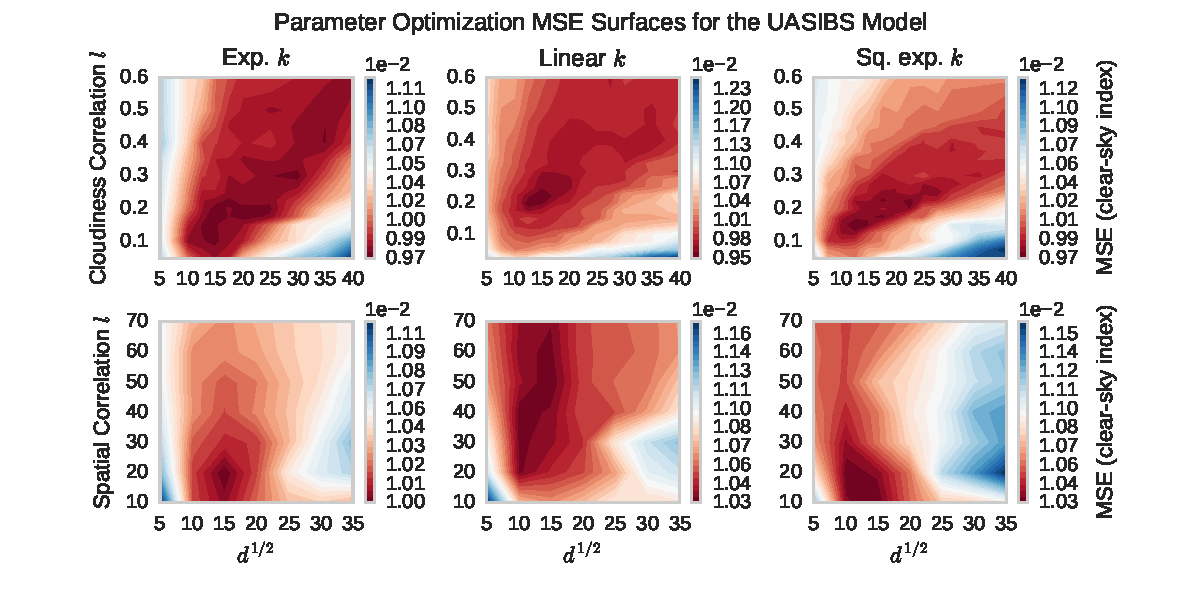
\includegraphics[width=1.05\textwidth]{figs/uasibs_optsurf.pdf}}
\vspace{-1em} \\
\subfloat{\hspace{-1em} 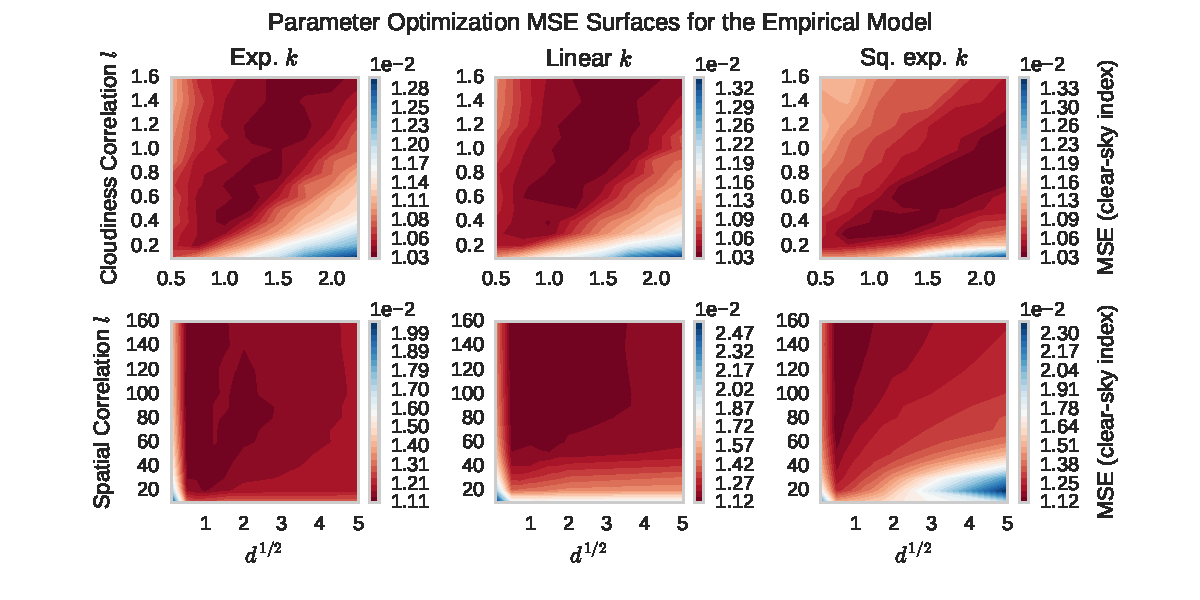
\includegraphics[width=1.05\textwidth]{figs/suny_optsurf.pdf}}
\caption[Optimization surfaces for OI parameters]{Optimization
  surfaces for the parameters $k,\: l,\: d$ of the optimal
  interpolation routine. The columns represent different choices of
  $k$, the rows distinguish between cloudiness and spatial
  correlation, the y-axis is $l$ and the x-axis is $d^{1/2}$. The top
  figure shows surfaces for the UASIBS model and the bottom is for the
  empirical model. Note, that for all choices of $k$ and the
  correlation parameterization, the surfaces for the UASIBS model have
  a clear minimum. The surfaces for the empirical model have less
  distinct minima indicating that optimal interpolation is not
  particularly sensitive to parameter choice for this model.}
\label{fig:paramopt}
\end{figure}


\section{Future Work}
(mainly pertaining to OI, mabye little bit of kalman)

new sat to irr algorithm

Here is some future work

How does NSRDB do?

GSIP?

GOES-16
%%% Local Variables:
%%% mode: latex
%%% TeX-master: "dissertation"
%%% End:
